
\subsection{Agreement between Model Electrical Features NeuroElectro Experiment Features}

\begin{markdown}
| Right | Left | Default | Center |
|------:|:-----|---------|:------:| 
|  12   |  12  |  12     |   12   | 
| 123   |  123 |   123   |  123   | 
|   1   |    1 |     1   |    1   | 
\end{markdown}




\begin{verbatim}
   chi\_square   p\_value
    2.125091  0.976935
\end{verbatim}


\setlength{\arrayrulewidth}{1mm}
\setlength{\tabcolsep}{18pt}
\renewcommand{\arraystretch}{2.5}

\begin{tabular}{ |p{3cm}||p{3cm}|p{3cm}|p{3cm}|  }
 \hline
 \multicolumn{4}{|c|}{Test Suite Results} \\
 \hline
 NeuroElectro Test Name & observations  & predictions & Z-score \\
 \hline
 RheobaseTest   & AF    &AFG&   004\\
 InputResistanceTest &   AX  & ALA   &248\\
 TimeConstantTest &AL & ALB&  008\\
 CapacitanceTest    &DZ & DZA&  012\\
 RestingPotential &   AS  & ASM&016\\
 APWidthTest & AD  & AND   &020\\
 APThresholdTes t& AO  & AGO&024\\
 \hline
\end{tabular}

            \begin{tcolorbox}[breakable, size=fbox, boxrule=.5pt, pad at break*=1mm, opacityfill=0]
\begin{Verbatim}[commandchars=\\\{\}]
                                         observations  \textbackslash{}
RheobaseTest                      213.849583333333 pA
InputResistanceTest             120.672073643411 Mohm
TimeConstantTest                  15.7342424242424 ms
CapacitanceTest                   150.584166666667 pF
RestingPotentialTest             -68.2481434599156 mV
InjectedCurrentAPWidthTest        1.20769387755102 ms
InjectedCurrentAPAmplitudeTest    80.4351020408164 mV
InjectedCurrentAPThresholdTest   -42.7357232704403 mV

                                              predictions    Z-Scores
RheobaseTest                             45.0439453125 pA     1.13318
InputResistanceTest             84.47885606885278 megaohm    0.444622
TimeConstantTest                    12.284367934517713 ms    0.450915
CapacitanceTest                      145.4135212781005 pF   0.0299731
RestingPotentialTest                 -68.3530583578185 mV   0.0128969
InjectedCurrentAPWidthTest          1.3100000000000003 ms     0.16468
InjectedCurrentAPAmplitudeTest       80.49511842343712 mV  0.00376319
InjectedCurrentAPThresholdTest       -38.5050967026868 mV    0.512854
\end{Verbatim}
\end{tcolorbox}
        
    \hypertarget{izhikevich-model-hippocampus-ca1-pyramidal-experiment.}{%
\section{Izhikevich model Hippocampus CA1 pyramidal
experiment.}\label{izhikevich-model-hippocampus-ca1-pyramidal-experiment.}}

            \begin{tcolorbox}[breakable, size=fbox, boxrule=.5pt, pad at break*=1mm, opacityfill=0]
\begin{Verbatim}
   chi\_square   p\_value
0    2.125091  0.976935
\end{Verbatim}
\end{tcolorbox}
        
            \begin{tcolorbox}[breakable, size=fbox, boxrule=.5pt, pad at break*=1mm, opacityfill=0]
\begin{Verbatim}
                                         observations  \textbackslash{}
RheobaseTest                                189.24 pA
InputResistanceTest             107.080327644332 Mohm
TimeConstantTest                  24.5021946169772 ms
CapacitanceTest                   89.7960714285714 pF
RestingPotentialTest             -65.2261863636364 mV
InjectedCurrentAPWidthTest        1.31895278450363 ms
InjectedCurrentAPAmplitudeTest     86.364525297619 mV
InjectedCurrentAPThresholdTest   -47.5985714285714 mV

                                              predictions   Z-Scores
RheobaseTest                           32.244873046875 pA   0.536865
InputResistanceTest             97.76274731515429 megaohm   0.100485
TimeConstantTest                     9.604335816193002 ms   0.717214
CapacitanceTest                      98.24126346645974 pF   0.133624
RestingPotentialTest                -65.55690901865944 mV  0.0554458
InjectedCurrentAPWidthTest          1.2000000000000002 ms    0.16846
InjectedCurrentAPAmplitudeTest       86.96668801838769 mV  0.0399524
InjectedCurrentAPThresholdTest      -39.99765398466066 mV    1.12315
\end{Verbatim}
\end{tcolorbox}
        

    

    \begin{center}
    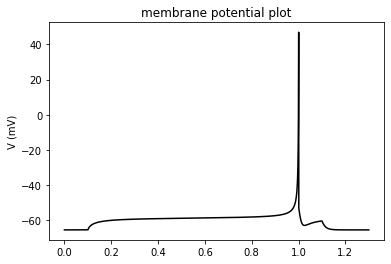
\includegraphics[]{notebooks_converted/make_normal_distribution_files/make_normal_distribution_8_2.png}
    \end{center}

    \hypertarget{conductance-based-model-hippocampus-ca1-pyramidal-experiment.}{%
\section{Conductance Based model Hippocampus CA1 pyramidal
experiment.}\label{conductance-based-model-hippocampus-ca1-pyramidal-experiment.}}

            \begin{tcolorbox}
            %[breakable, size=fbox, boxrule=.5pt, pad at break*=1mm, opacityfill=0]
\begin{Verbatim}[commandchars=\\\{\}]
   chi\_square   p\_value
0   17.216463  0.027932
\end{Verbatim}
\end{tcolorbox}
        
    

            \begin{tcolorbox}[breakable, size=fbox, boxrule=.5pt, pad at break*=1mm, opacityfill=0]
\begin{Verbatim}[commandchars=\\\{\}]
   chi\_square   p\_value
0   17.216463  0.027932
\end{Verbatim}
\end{tcolorbox}
        
            \begin{tcolorbox}[breakable, size=fbox, boxrule=.5pt, pad at break*=1mm, opacityfill=0]
\begin{Verbatim}[commandchars=\\\{\}]
   RheobaseTest  InputResistanceTest  TimeConstantTest  CapacitanceTest  \textbackslash{}
0      0.104364              0.26776          0.909698         0.779279

   RestingPotentialTest  InjectedCurrentAPWidthTest  \textbackslash{}
0              0.263258                    2.539904

   InjectedCurrentAPAmplitudeTest  InjectedCurrentAPThresholdTest
0                        0.197484                        3.023183
\end{Verbatim}
\end{tcolorbox}
        
            \begin{tcolorbox}[breakable, size=fbox, boxrule=.5pt, pad at break*=1mm, opacityfill=0]
\begin{Verbatim}[commandchars=\\\{\}]
                                         observations  \textbackslash{}
RheobaseTest                                189.24 pA
InputResistanceTest             107.080327644332 Mohm
TimeConstantTest                  24.5021946169772 ms
CapacitanceTest                   89.7960714285714 pF
RestingPotentialTest             -65.2261863636364 mV
InjectedCurrentAPWidthTest        1.31895278450363 ms
InjectedCurrentAPAmplitudeTest     86.364525297619 mV
InjectedCurrentAPThresholdTest   -47.5985714285714 mV

                                               predictions  Z-Scores
RheobaseTest                                      225.0 pA  0.104364
InputResistanceTest             130.26055973925207 megaohm   0.26776
TimeConstantTest                      6.518945502058039 ms  0.909698
CapacitanceTest                       50.04542829469856 pF  0.779279
RestingPotentialTest                -63.787552448611955 mV  0.263258
InjectedCurrentAPWidthTest                         0.25 ms    2.5399
InjectedCurrentAPAmplitudeTest        89.14231395773962 mV  0.197484
InjectedCurrentAPThresholdTest      -62.833162761594465 mV   3.02318
\end{Verbatim}
\end{tcolorbox}
        
    \begin{center}
    \adjustimage{max size={0.9\linewidth}{0.9\paperheight}}{make_normal_distribution_files/make_normal_distribution_18_0.png}
    \end{center}
    { \hspace*{\fill} \\}
    
    \hypertarget{adaptive-exponential-model-hippocampus-ca1-pyramidal-experiment.}{%
\section{Adaptive Exponential Model Hippocampus CA1 pyramidal
Experiment.}\label{adaptive-exponential-model-hippocampus-ca1-pyramidal-experiment.}}

    
    \begin{verbatim}
<Figure size 432x288 with 0 Axes>
    \end{verbatim}

    
    \begin{center}
    \adjustimage{max size={0.9\linewidth}{0.9\paperheight}}{make_normal_distribution_files/make_normal_distribution_21_1.png}
    \end{center}
    { \hspace*{\fill} \\}
    
            \begin{tcolorbox}[breakable, size=fbox, boxrule=.5pt, pad at break*=1mm, opacityfill=0]
\begin{Verbatim}[commandchars=\\\{\}]
                    0
chi\_square  10.232514
p\_value      0.249084
\end{Verbatim}
\end{tcolorbox}
        
            \begin{tcolorbox}[breakable, size=fbox, boxrule=.5pt, pad at break*=1mm, opacityfill=0]
\begin{Verbatim}[commandchars=\\\{\}]
   RheobaseTest  InputResistanceTest  TimeConstantTest  CapacitanceTest  \textbackslash{}
0      0.104364              0.26776          0.909698         0.779279

   RestingPotentialTest  InjectedCurrentAPWidthTest  \textbackslash{}
0              0.263258                    2.539904

   InjectedCurrentAPAmplitudeTest  InjectedCurrentAPThresholdTest
0                        0.197484                        3.023183
\end{Verbatim}
\end{tcolorbox}
        
            \begin{tcolorbox}[breakable, size=fbox, boxrule=.5pt, pad at break*=1mm, opacityfill=0]
\begin{Verbatim}[commandchars=\\\{\}]
                                         observations  \textbackslash{}
RheobaseTest                                189.24 pA
InputResistanceTest             107.080327644332 Mohm
TimeConstantTest                  24.5021946169772 ms
CapacitanceTest                   89.7960714285714 pF
RestingPotentialTest             -65.2261863636364 mV
InjectedCurrentAPWidthTest        1.31895278450363 ms
InjectedCurrentAPAmplitudeTest     86.364525297619 mV
InjectedCurrentAPThresholdTest   -47.5985714285714 mV

                                               predictions  Z-Scores
RheobaseTest                                      225.0 pA  0.104364
InputResistanceTest             130.26055973925207 megaohm   0.26776
TimeConstantTest                      6.518945502058039 ms  0.909698
CapacitanceTest                       50.04542829469856 pF  0.779279
RestingPotentialTest                -63.787552448611955 mV  0.263258
InjectedCurrentAPWidthTest                         0.25 ms    2.5399
InjectedCurrentAPAmplitudeTest        89.14231395773962 mV  0.197484
InjectedCurrentAPThresholdTest      -62.833162761594465 mV   3.02318
\end{Verbatim}
\end{tcolorbox}
        
    \hypertarget{olfactory-mitral-cell-experiment-izhikevich-model}{%
\section{Olfactory Mitral Cell Experiment/ Izhikevich
Model}\label{olfactory-mitral-cell-experiment-izhikevich-model}}

            \begin{tcolorbox}[breakable, size=fbox, boxrule=.5pt, pad at break*=1mm, opacityfill=0]
\begin{Verbatim}[commandchars=\\\{\}]
                   0
chi\_square  2.019044
p\_value     0.980422
\end{Verbatim}
\end{tcolorbox}
        
            \begin{tcolorbox}[breakable, size=fbox, boxrule=.5pt, pad at break*=1mm, opacityfill=0]
\begin{Verbatim}[commandchars=\\\{\}]
   InputResistanceTest  TimeConstantTest  CapacitanceTest  \textbackslash{}
0             0.209574          0.178053         0.030453

   RestingPotentialTest  InjectedCurrentAPWidthTest  \textbackslash{}
0              0.297853                     0.19034

   InjectedCurrentAPAmplitudeTest  InjectedCurrentAPThresholdTest
0                        0.035634                        1.347693
\end{Verbatim}
\end{tcolorbox}
        
            \begin{tcolorbox}[breakable, size=fbox, boxrule=.5pt, pad at break*=1mm, opacityfill=0]
\begin{Verbatim}[commandchars=\\\{\}]
                                         observations  \textbackslash{}
InputResistanceTest             130.083333333333 Mohm
TimeConstantTest                  24.4833333333333 ms
CapacitanceTest                             235.75 pF
RestingPotentialTest                    -58.140625 mV
InjectedCurrentAPWidthTest                    1.61 ms
InjectedCurrentAPAmplitudeTest                68.4 mV
InjectedCurrentAPThresholdTest               -38.9 mV

                                               predictions   Z-Scores
InputResistanceTest             111.76440601217192 megaohm   0.209574
TimeConstantTest                     26.351190325249217 ms   0.178053
CapacitanceTest                      235.77444076765715 pF  0.0304534
RestingPotentialTest                 -59.78177430465574 mV   0.297853
InjectedCurrentAPWidthTest                         1.54 ms    0.19034
InjectedCurrentAPAmplitudeTest         68.6158436132009 mV  0.0356342
InjectedCurrentAPThresholdTest      -30.452468089353545 mV    1.34769
\end{Verbatim}
\end{tcolorbox}
        
    \hypertarget{neocortex-pyramidal-experiment-conductance-based-model}{%
\section{Neocortex Pyramidal Experiment Conductance based
model}\label{neocortex-pyramidal-experiment-conductance-based-model}}

    \hypertarget{cerebellum-purkinje-cell-experiment-conductance-izhikevich-model}{%
\section{Cerebellum Purkinje cell Experiment Conductance Izhikevich
Model}\label{cerebellum-purkinje-cell-experiment-conductance-izhikevich-model}}

    \begin{Verbatim}[commandchars=\\\{\}]
INFO:\_\_main\_\_:gen       nevals  avg     std     min     max
1       25      279.541 609.858 9.86573 2489.8
gen     nevals  avg     std     min     max
1       25      279.541 609.858 9.86573 2489.8
    \end{Verbatim}

    
    \begin{verbatim}
HBox(children=(FloatProgress(value=0.0, max=200.0), HTML(value='')))
    \end{verbatim}

